\subsection{Dimensional Analysis and Scaling Laws}
\label{sec:dimensional}

A Buckingham Pi analysis of the fluid-filled viscoelastic shell identifies
eight independent dimensionless groups from the eleven governing variables
(Table~\ref{tab:pi_groups}).  For flexural modes ($n \ge 2$), the fluid bulk
modulus $K_f$ contributes no stiffness and the loss tangent $\eta$ affects
only damping, reducing the effective parameter count to six: a dimensionless
frequency output $\Pi_0$ governed by five input groups.  The scaling law
takes the closed form
\begin{equation}
  f_n = \frac{1}{2\pi}\sqrt{\frac{E}{\rho_f}}\,\frac{1}{a}\;
        \Phi_n\!\left(\frac{h}{a},\;\frac{c}{a},\;
        \frac{\rho_w}{\rho_f},\;\frac{P_\mathrm{iap}}{E},\;\nu\right),
  \label{eq:scaling_law}
\end{equation}
where $\Phi_n$ admits a closed-form expression from the shell equations
(see supplementary material).  All 486 points of the parametric study
collapse onto the analytical curves with a maximum relative error of
5.8e-16 (Figure~\ref{fig:collapse}), confirming that the ten-parameter
space reduces to five governing groups.

\begin{table}[htbp]
  \centering
  \caption{Dimensionless groups from Buckingham Pi theorem.  Groups marked
  $\ast$ drop out of the flexural-mode frequency.}
  \label{tab:pi_groups}
  \begin{tabular}{clll}
    \hline
    Group & Definition & Name & Role \\
    \hline
    $\Pi_0$ & $f_n\, a\sqrt{\rho_f/E}$ & dimensionless frequency & output \\
    $\Pi_1$ & $h/a$ & thickness ratio & stiffness \& mass \\
    $\Pi_2$ & $c/a$ & aspect ratio & geometry \\
    $\Pi_3$ & $\rho_w/\rho_f$ & density ratio & added mass \\
    $\Pi_4^\ast$ & $K_f/E$ & compressibility ratio & breathing mode only \\
    $\Pi_5$ & $P_\mathrm{iap}/E$ & prestress ratio & tension stiffening \\
    $\Pi_6$ & $\nu$ & Poisson's ratio & membrane coupling \\
    $\Pi_7^\ast$ & $\eta$ & loss tangent & damping only \\
    \hline
  \end{tabular}
\end{table}

\begin{figure}[htbp]
  \centering
  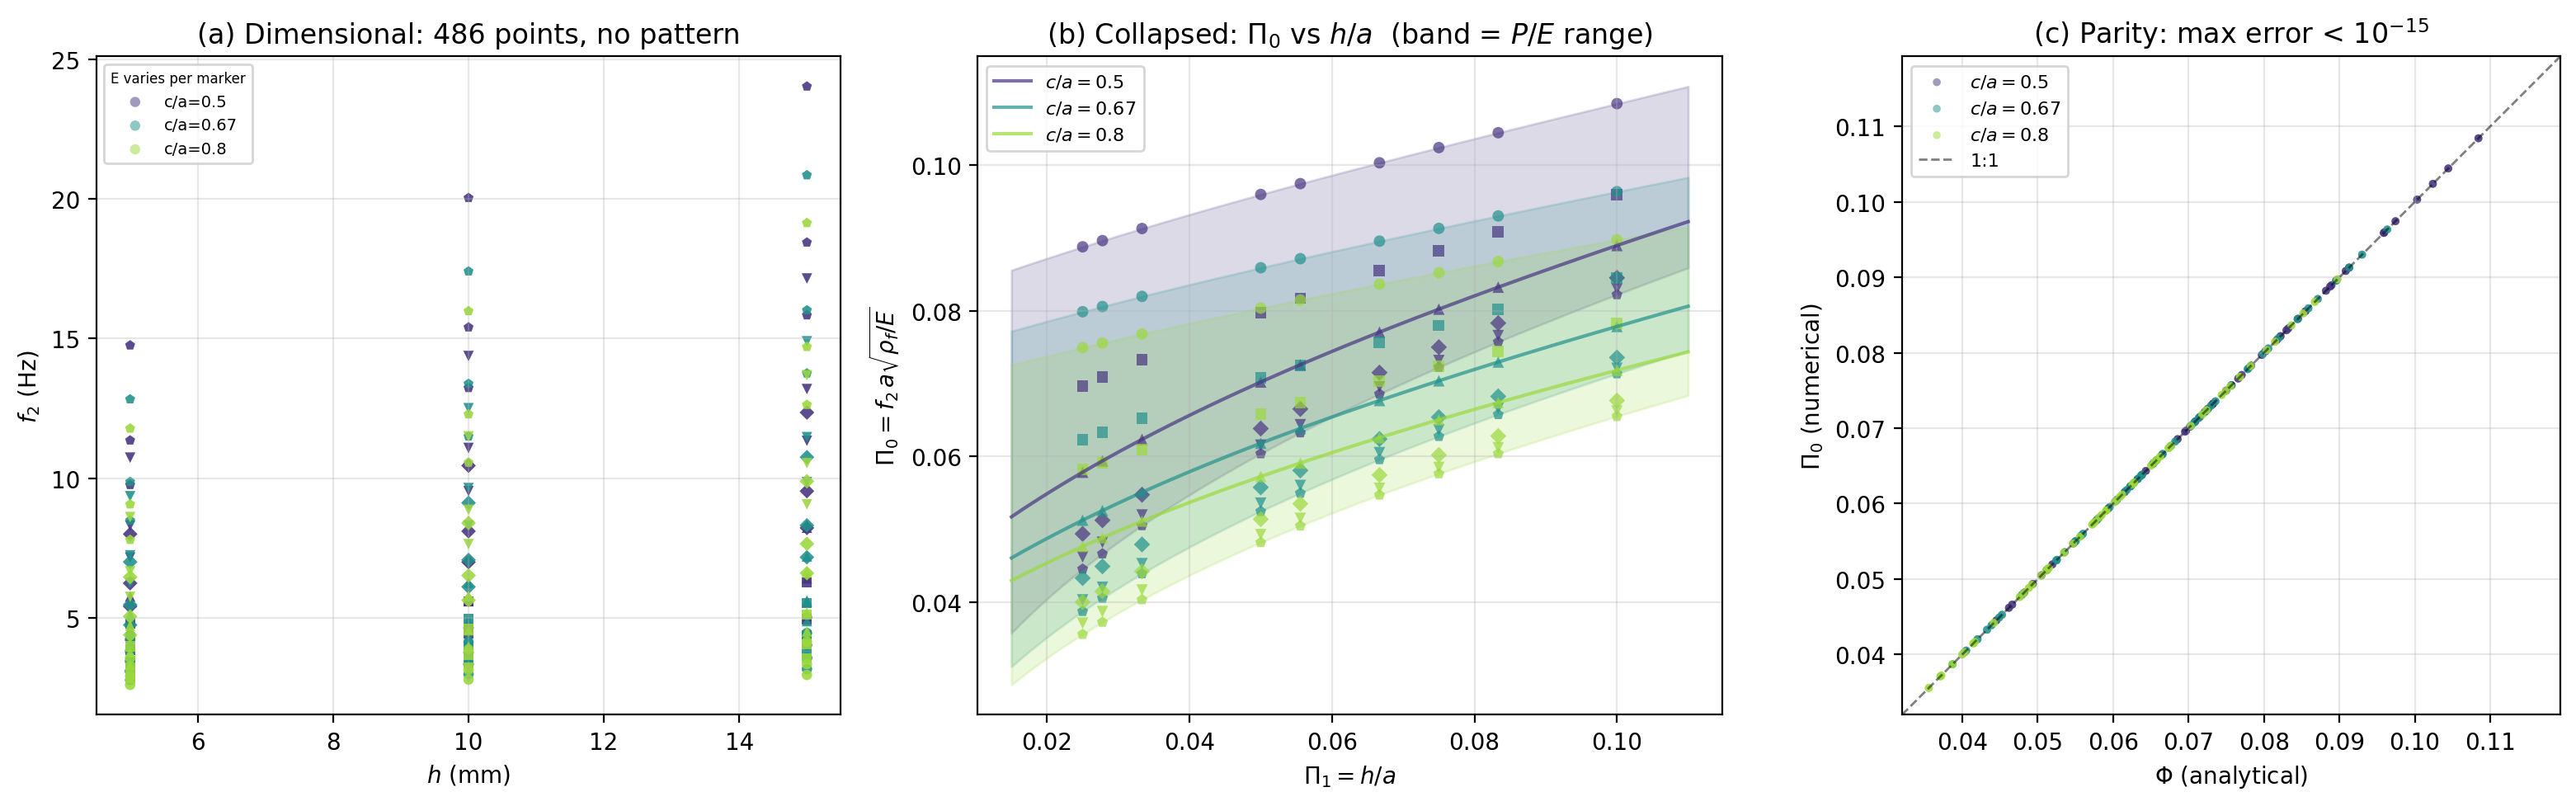
\includegraphics[width=\textwidth]{../data/figures/fig_dimensional_collapse.png}
  \caption{Dimensional collapse of the 486-point parametric study.
  \emph{(a)}~Raw dimensional data ($f_2$ vs.\ $h$) shows no clear pattern.
  \emph{(b)}~Non-dimensionalising via equation~\eqref{eq:scaling_law} collapses
  all points onto universal curves $\Pi_0(h/a)$ parameterised by $c/a$; shaded
  bands span the $P_\mathrm{iap}/E$ range, different markers denote different $E$.
  \emph{(c)}~Parity plot confirms the analytical $\Phi$ reproduces every
  numerical point to machine precision.}
  \label{fig:collapse}
\end{figure}

Cross-species scaling follows directly from~\eqref{eq:scaling_law}: if two
organisms share similar $\Pi$-group values, their resonant frequencies scale
as $f \propto (1/a)\sqrt{E/\rho_f}$.  Because smaller animals have both
smaller $a$ and lower $E$ (softer tissue), the net frequency shift is less
than a pure $1/a$ law.  Table~\ref{tab:scaling} lists predictions for four
species.  The airborne coupling coefficient $(ka)^2$ is of order $10^{-4}$
for all species, making the mechanical-to-airborne coupling ratio
$\mathcal{R} \sim 10^{3}\text{--}10^{4}$ roughly size-independent.  This
validates the use of animal models for abdominal resonance studies, provided
excitation is delivered mechanically rather than acoustically.  The breathing
mode ($n=0$), dominated by $K_f$, would require a body radius of order
\SI{410}{\metre} to reach \SI{20}{\hertz}; it never enters
the infrasound range for any biological organism.

\begin{table}[htbp]
  \centering
  \caption{Cross-species scaling of the $n=2$ flexural mode.
  Here $\mathcal{R} = 1/(ka)^2$ is the radiation-efficiency scaling,
  which isolates the geometric acoustic mismatch.
  This differs from the displacement ratio
  $\mathcal{R} \approx 6.6 \times 10^4$
  in Eq.~\eqref{eq:coupling_ratio}, which compares physical
  displacements at matched excitation levels
  (\SI{120}{\decibel} SPL airborne vs.\
  \SI{0.1}{\metre\per\second\squared} mechanical).}
  \label{tab:scaling}
  \begin{tabular}{lccccc}
    \hline
    Species & $a$ (cm) & $f_2$ (Hz) & $\Pi_0$ & $ka$ & $\mathcal{R}$ \\
    \hline
    Rat & 3 & 15.7 & 0.0673 & 7.7e-03 & 1.7e+04 \\
    Cat & 8 & 7.2 & 0.0646 & 9.3e-03 & 1.2e+04 \\
    Pig & 15 & 4.5 & 0.0686 & 1.1e-02 & 8.6e+03 \\
    Human & 18 & 3.9 & 0.0717 & 1.1e-02 & 7.7e+03 \\
    \hline
  \end{tabular}
\end{table}

\begin{figure}[htbp]
  \centering
  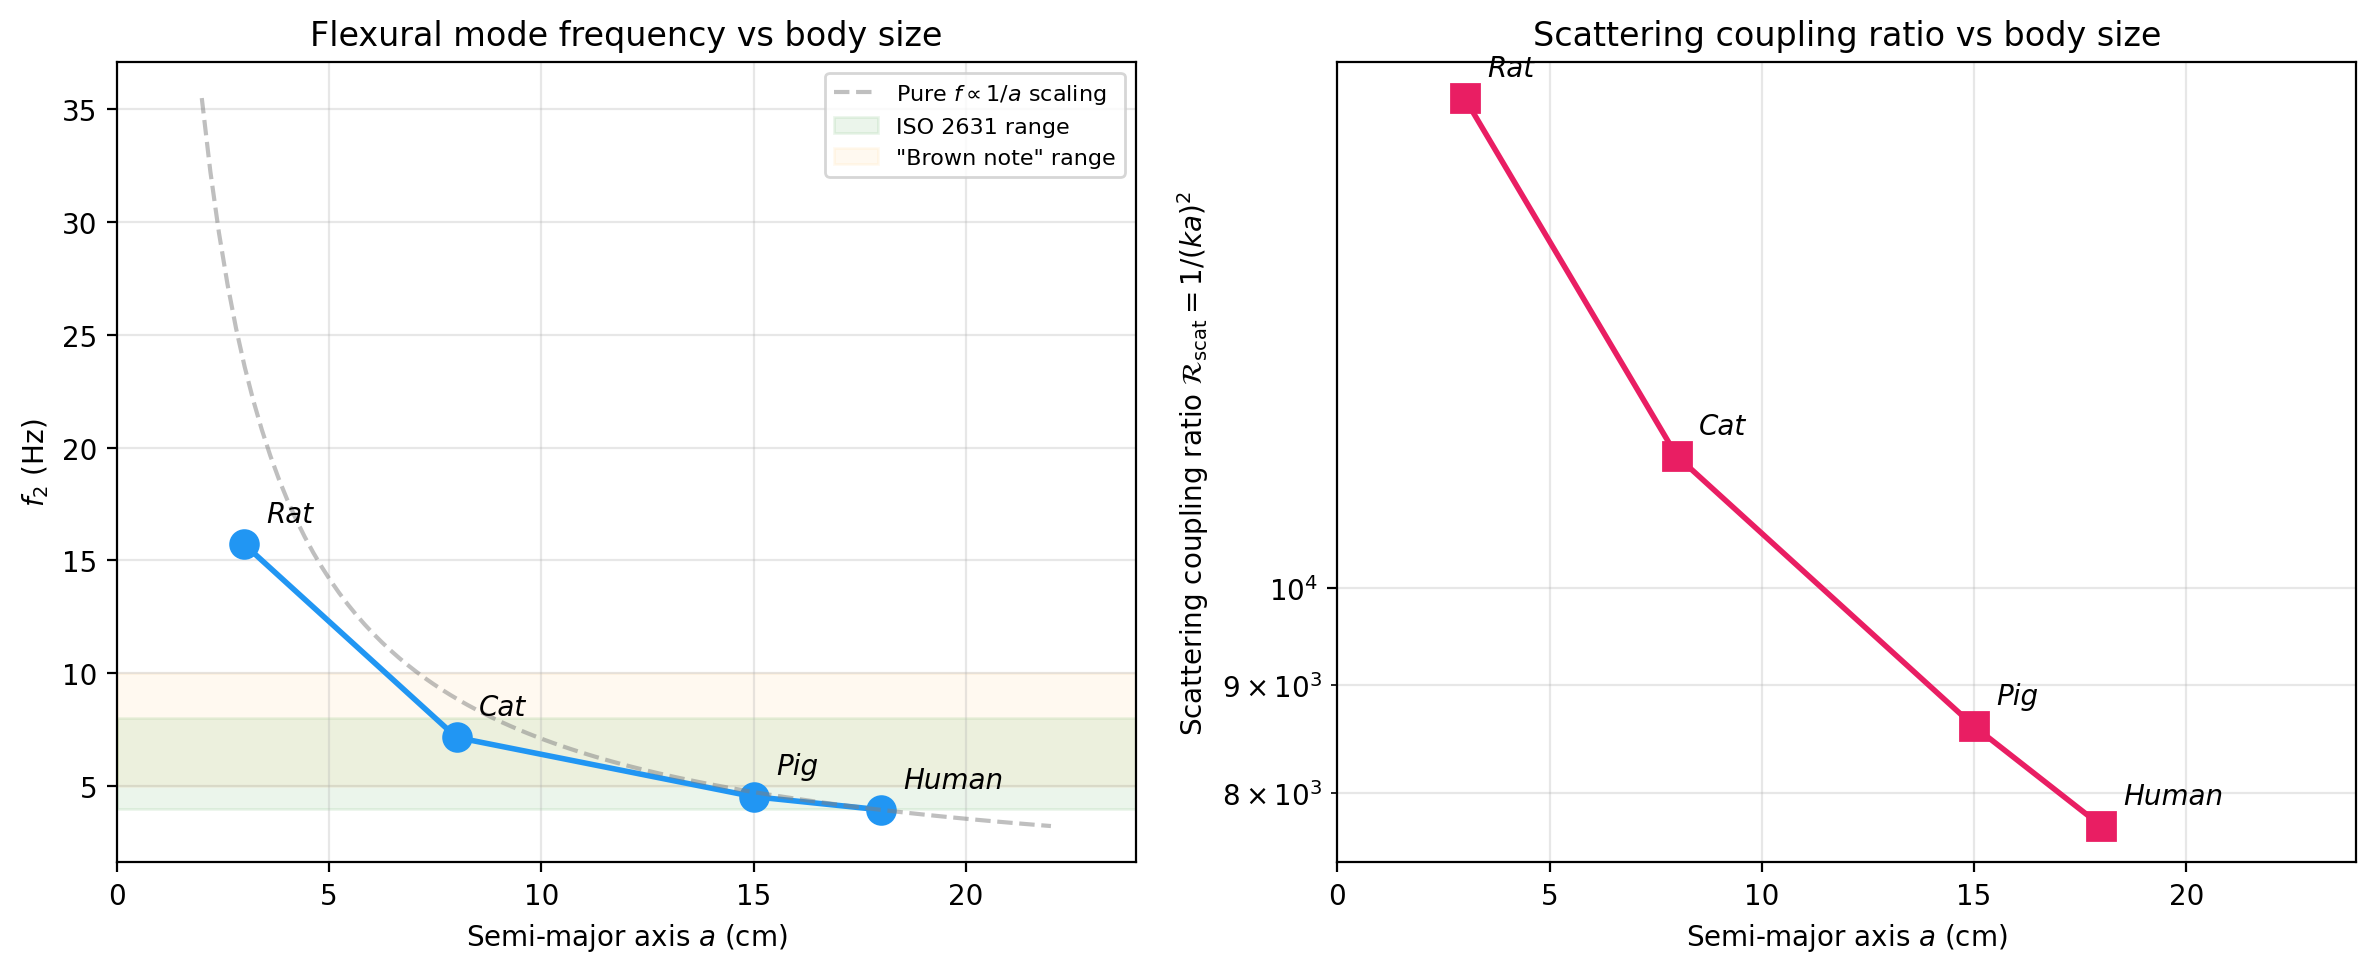
\includegraphics[width=\textwidth]{../data/figures/fig_scaling_law.png}
  \caption{Cross-species scaling.
  \emph{Left:} Flexural mode $f_2$ vs.\ semi-major axis $a$.  The dashed
  line shows pure $1/a$ scaling; deviations arise because smaller animals
  have softer tissue and different $h/a$.
  \emph{Right:} Coupling ratio $\mathcal{R}$ is approximately
  size-independent, supporting the validity of animal-model extrapolation.}
  \label{fig:scaling_law}
\end{figure}
